
\section{Results}
\label{sec:result}

\subsection{Statistical Procedure }
\label{sec:limits}
The statistical interpretation of data in the presented search is based on profiled likelihood ratio test statistic used
for the Higgs boson searches~\cite{lhclimits}. The statistical procedures described in the 
following are implemented in the software packages described in~\cite{roofit,roostat,histfactory}.

\subsubsection{The Likelihood Function}
The statistical interpretation of data is performed by means of testing the compatibility
of the \textit{background only}  and and the \textit{signal-plus-background}  hypotheses with the observed data.  
%Statistical tests are used to quantify the significance of an observation or to set an exclusion limits, 
%in a search for new phenomena, hypothesis testing is performed by means of two hypothesis: 
%the \textit{background only} $H_0$ and and the \textit{signal-plus-background} $H_1$ hypothesis.  
The main ingredient of the hypothesis \emph{test statistic}, defined later on in this section,  
is a binned likelihood function for the data set, $\mathcal{D}$:
\begin{equation}\label{likelihood}
\mathcal{L}(\mathcal{D}~|~\mu, \boldsymbol{\theta}) = \text{Pois(}\mathcal{D}~ |~ \mu \cdot s(\boldsymbol{\theta}) 
	+ b(\boldsymbol{\theta})) \cdot \prod_{j,i}\mathcal{G}(\theta_j^{sys} ~ | ~ 0, 1) \cdot \Gamma(\theta^{stat}_i | \beta_i)
\end{equation}
describing how likely is a certain hypotesis given the observation of the data set $\mathcal{D}$.
The signal strenght modifier $\mu$ allows for reproducing a continuous set of signal hypotheses with 
different cross-section. The value of $\mu= 0$ corresponds to the background-only hypothesis. 
The vector $\boldsymbol{\theta}$ represents the set of \emph{nuisance} parameters  related to
the systematic ($\theta_j^{sys}$) and to the statistical ($\theta^{stat}_i$) 
uncertainties of the background and signal predictions. 
The functions s($\boldsymbol{\theta}$) and  b($\boldsymbol{\theta}$)
represent the expected signal and background distribution, respectively, these are binned histograms
of the invariant \mmc mass distributions.
The function $\mathcal{G}(\theta_j^{sys} ~ | ~ 0, 1)$
is the  Gaussian\footnote{Evaluation of systematic uncertainties is obtained from from auxiliary measurements, from Bayes theorem,
	assuming a flat prior and a Gaussian distribution for the measured parameter a Gaussian posterior is obtained.	
}
probability density function (p.d.f.) for the nuisance parameter $\theta_j^{sys}$, 
which is assumed to be distributed with mean~=~0 and $\sigma = 1$.  The impact of the corresponding systematic uncertainty
on the  signal and backgrounds yields and on the shape of the \mmc invariant mass distribution
 is evaluated separately as described in Section~\ref{sec:Systematics}.
The function  $\Gamma(\theta^{stat}_i | \beta_i)$ is an extended gamma function\footnote{The posterior of a
	Poisson distribution assuming a flat prior is a gamma function}
describing the p.d.f. for the nuisance parameter $\theta^{stat}_i$ related 
to the statistical uncertainty $ \beta_i$, for the bin $i$ of the histogram.
Each value of the nuissance parameter set $\boldsymbol{\theta}$ is associated with a variation of the predicted
signal and background event yields with respect to the nominal prediction.
%are evaluated represent
%the uncertainties on the signal and background yields,  or mass shape of the analysis, those uncertainties 
%are usually measured by auxiliary measure to the analysis, like JES for example, or come from theory uncertainty,
%the single p.d.f. of the parameter $\theta_i$ is assumed Gaussian distributed 
%where and it is only function of the parameter $\mu$ and of the
%nuisance parameter $\boldsymbol{\theta}$. If the hypothesis under test is unlikely to happen with the given dataset the value of 
%$\mathcal{L}$ is decreasing,
%one can define which is the best value of a parameter that describes the data via maximizing the likelihood,
%obtaining a so called maximum likelihood estimator. 
The Poisson distribution in equation~\eqref{likelihood} is a binned p.d.f. and 
stands for a product of Poisson probabilities to observe $n_i$ events in the bin \textit{i} of the \mmc histogram:
$$
 \text{Pois(}\mathcal{D} ~ | ~ \mu \cdot s(\boldsymbol{\theta}) + b(\boldsymbol{\theta})) = \prod_{i} \frac{(\mu s_i(\boldsymbol{\theta}) +b_i(\boldsymbol{\theta}))^{n_i}}{n_i!} ~ e^{-\mu s_i(\boldsymbol{\theta}.)
 -b_i(\boldsymbol{\theta})}
$$
The \mmc mass distributions in the b-tagged and b-vetoed category are analyzed separately.
The actual implementation in the likelihood function of the ABCD method follows that suggested in~\cite{ABCD}
and it is described in more detail in Appendix~\ref{appendix:limit}.

\subsubsection{Statistical Combination of Results From Two Event Categories}
Complementary event categories in one search channel, 
like the b-tagged and b-vetoed event categories, 
can be combined in order to increase the
sensitivity to the signal. If there are no events entering both categories, as is the case for  the presented analysis,
the statistical combination is the product of the likelihood
functions for the individual categories. For the combination, the  convention described in~\cite{lhclimits} is used
to take into account the correlation between different sources of uncertainties.
Uncertainties are considered either as fully correlated, which means that the same nuisance parameter
is describing the given systematic effect in both categories,  or fully uncorrelated, in which case different nuisance parameter are
employed in the two categories. Partially correlated uncertainties are either slit into component which are fully
or uncorrelated or they are defined as  to either fully correlated or uncorrelated.
The choice of the above options is made by always selecting the most conservative assumptin.



\subsubsection{The Test Statistic and the Exclusion Limits}
To compute the compatibility of the data with a given hypothesis a test statistic is defined based on the
\emph{profiled likelihood ratio}~\cite{Asympt}: 
\begin{equation}
\tilde{q_{\mu}} ~ = ~ -2 \text{ln} ~ \frac{\mathcal{L}(\mathcal{D}~|~\mu, \hat{\boldsymbol{\theta}}_{\mu})}{\mathcal{L}(\mathcal{D} ~| ~ 
\hat{\mu}, \hat{\boldsymbol{\theta}})}
\quad \text{with the constraint} \quad 0 \leq \hat{\mu} \leq \mu.
\end{equation}
$\mathcal{L}$ is the likelihood function defined in equation~\eqref{likelihood}, $\hat{\mu}$ and $\hat{\boldsymbol{\theta}}$ 
are the global maximum likelihood estimators for $\mu$ and $\boldsymbol{\theta}$ given the data, 
whereas $\hat{\boldsymbol{\theta}}_{\mu}$ is the maximum likelihood estimator of $\boldsymbol{\theta}$ given the data but  with
a signal strength fixed to the value of $\mu$. $\tilde{q_{\mu}}$ is increasing with 
increasing disagreement between data and the given hypothesis with a signal strenght $\mu$.
Based on this, the procedure for setting upper exclusion limits on the signal cross-section
is defined as follows:
\begin{enumerate}
%	\item The signal hypothesis with signal strength $\mu$ is assumed, under this assumption a set of MC 
%	\textit{pseudo-data} is generated for different values of $\mu$.
%
%	\item  $\tilde{q_{\mu}}$ is calculated for each of the \textit{pseudo-dataset} and each signal hypothesis generating
%	the expected probability density function for $\tilde{q_{\mu}}$ given $\mu$, 
%	$\text{f}(\tilde{q_{\mu}} ~| ~ \mu, \hat{\boldsymbol{\theta}}_{\mu},H_1)$.
%
%	\item The same procedure is repeated for the null hypothesis: pseudo-data are generated with the distribution 
%	of background only and 	obtain  the $\text{f}(\tilde{q_{\mu}} ~ | ~ \mu = 0, \hat{\boldsymbol{\theta}}_{0}, H_0)$.
%
	\item The probability density function of $\tilde{q_{\mu}}$ is determined  under the background-only ($H_0$) and 
	the  signal-plus-background ($H_{\mu}$) hypotheses for any given value of $\mu$.
	Since the determination of these distributions by means of pseudo-data demands large computing time,
	asymptotic approximation formulas described in~\cite{Asympt} are employed.
	

	\item Once the p.d.f. for the background-only and signal-plus-background hypothesis are obtained, 
	it is possible to define for a given dataset  two probability values (p-values) for any given value of $\mu$.
	These are the probabilities to observe data less compatible with the considered hypothesis than the 
	actual observation:
	$$
	p_{s+b} = P(\tilde{q_{\mu}} > \tilde{q_{\mu}}^{observed} ~ | ~ H_{\mu})  
	$$
	$$ 
	p_{b} = P(\tilde{q_{\mu}} > \tilde{q_{\mu}}^{observed} ~ | ~ H_0)
	$$
	The ratio of this two probabilities defines the quantity $CL_{s} = p_{s+b} / p_{b}$ \cite{cls1,cls2}.

	\item If for a given $\mu$ the $CL_{s}$ value of $CL_{s} ~ \leq ~ \alpha $ is obtained, the signal-plus-background
	 hypothesis (with the corresponding $\mu$ value)  is considered to be 
	 excluded at a (1 - $\alpha$) $CL_{s}$ confidence level. The 95\% confidence level upper limit on $\mu$,
	denoted as $\mu^{95\%}$, is defined as the smallest value of $\mu$ for which the  $CL_{s}$ value is no longer 
	greather than  $0.05\,.$
\end{enumerate}
%This is a quite complicated prescription, however 
%its interpretation is not so different from the usual Neyman Construction~\cite{} of confidence intervals:
%for each $\mu$ is possible to define $\tilde{q_{\mu}}^{95}$ for which the probability 
%P$(\tilde{q_{\mu}} \geq \tilde{q_{\mu}}^{95} ~ |~ \mu, ~ H_1$) = 5\%, this means that if $H_1$ is true one expects 
%$\tilde{q_{\mu}} \geq \tilde{q_{\mu}}^{95}$ in 5\% of the cases. With this definition $\mu^{95}$ would be the value of $\mu$
%that for the observed data gives $\tilde{q_{\mu}} = \tilde{q_{\mu}}^{95}$, or in other words a p-value of 5\%.
By construction, rejecting all values of $\mu > \mu^{95\%}$, the signal-plus-background hypothesis will be 
rejected when it is true at most 5\% of the time.
%given the fact that $\tilde{q_{\mu}}$ is increasing with increasing discrepancy of the hypothesis with data.
The $CL_{s}$ prescription is a conservative approach protecting the signal exclusion upper limit from  downward  fluctuation of the data.
% For each pseudo-data sample one can calculate then $\mu^{95}$, which is the biggest value of $\mu$ which gives $\tilde{q_{\mu}} > \tilde{q_{\mu}}^{95}$
%
% Generate a large set of pseudo-data under the hypothesis $H_{0}$ and calculate  $\mu^{95}$ for each of them, by construction one would have
%	that if $H_1$ is true for $\mu > \mu^{95}$ one has $\tilde{q_{\mu}} > \tilde{q_{\mu}}^{95}$ only 5\% of the cases.
%	
%So one it is said that the $\mu > \mu^{95}$ are excluded by data under the hypothesis $H_1$ at 95\% of Confidence Level, meaning that 
%for value of $\mu > \mu^{95}$  one would reject the $H_1$ when is true at most 5\% of the time. 
%
The expected median exclusion upper-limit and its error are evaluated with the procedure described above under the background-only hypothesis.
The obtained results have been cross-checked using generated pseudo-data instead of the asymptotic approximation for the determination
of the $\tilde{q_{\mu}}$ probability density functions. 


\subsection{Exclusion Limits on the Signal Production}
The procedure described in section~\ref{sec:limits} is  the one used for the SM Higgs, for the MSSM further complication
arises: one has to consider in the signal 
model three Higgs, in a particular scenario the masses and cross section are defined for a given point in the $\tan \beta - m_A$
plane, so the procedure described previously has to be repeated for each point in that plane. 
%For a given scenario, 
%a point in the  $\tan \beta - m_A$ plane is excluded with 95\% $CL_{s}$ confidence level if $\mu^{95} \leq 1$ for that point. 
%Only a limited number of $\tan \beta - m_A$ points are generated, 
%a linear interpolation is used to determine the $\tan \beta$ excluded for a given $m_A$.
For the $m_h^{max}$ scenario exclusion limits are derived by calculating $95\%$ CLs limits on the cross section of
$bb$/$gg\to A$/$H$/$h\to\tau_{lep}\tau_{lep}$ for 15 tan$\beta$ values (between\footnote{The set of  tan$\beta$ values used
is 5, 8, 10, 13, 16, 20, 23, 26, 30, 35, 40, 45, 50, 55, 60}  $\mathrm{tan}\beta=5$ and $\mathrm{tan}\beta=60$),
a point in the  $\tan \beta - m_A$ plane is excluded if $\mu^{95} \leq 1$ for that point, 
a linear interpolation is used to determine the $\tan \beta$ excluded for a given $m_A$.
The procedure is followed for a set of different CP-odd Higgs masses $m_A$: 90, 100, 110, 120, 125, 130,
140, 150, 170, 200, 250 and 300 GeV.
The event yield has been compared between data and background expectation in bins of the \mmc distribution. The bin sizes were chosen
such that there are enough events left for the asymptotic approximation  to  hold.
Table~\ref{table:final_numbers} compares yields between data and background model for the two categories at the final
stage of the cut flow. Additionally, figure \ref{fig:mmc_categories} shows the \mmc distributions after the full 
selections of b-tagged and b-vetoed categories. 

\begin{table} [t]
\centering
\begin{tabular}{c p{0.5cm} r l l p{1cm} r l l }
\hline
\hline
Sample 	&	& \multicolumn{3}{c}{b-tagged category} 		&	& \multicolumn{3}{c}{b-vetoed category} 		\\ 	[0.5ex]
		&	&  N(event)	&	Stat.	&Syst.  & 	&  N(event)	&  Stat.	& Syst.		\\ [0.5ex]	
\hline
\Ztautau        &     	&       418  	&    $\pm$ 6	&	&       & 54680		& $\pm$ 60	&  		\\   [0.5ex]
\ttbar          &       &       330   	&    $\pm$ 10	&       &       & 2228		& $\pm$ 25	&	  	\\  [0.5ex]
Multi-jet        &       &       100	&    $\pm$ 15	&       &       & 3940		& $\pm$ 330	&	  	\\  [0.5ex]
\Wlnu           &       &       10      &    $\pm$ 6    &       &       & 650		& $\pm$ 100	&	  	\\  [0.5ex]
Dibosons         &       &       13.1    &    $\pm$ 1.8  &       &       & 2921		& $\pm$ 27	&	  	\\  [0.5ex]
Single Top      &       &       90	&    $\pm$ 6    &       &       & 443		& $\pm$ 15	&	  	\\  [0.5ex]
\Zll            &       &       0.9     &    $\pm$ 0.8  &       &       & 430		& $\pm$ 40	&	  	\\  [0.5ex]
Total           &       &       962     &    $\pm$ 16 	&       &       & 65290		& $\pm$ 180	&	  	\\  [0.5ex]
\hline
Signal  	&	&		& 		&	&	&		&		&		\\	[0.5ex]
\hline
Data	        &	& -		& - 		& -	& 	&	-	&	-	&	-	\\	[0.5ex]
\hline
\hline

\end{tabular}
\caption{Comparison between yield in data and the one expected from the background model, 
	b-tagged and b-vetoed category are reported separately. }
\label{table:final_numbers}
\end{table}

\begin{figure}[tp]
     \begin{center}
     \subfigure[]{		
            \includegraphics[page=6,width=0.47\textwidth]{figure/std_plots_mass.pdf}
	    \label{fullbtag2}	
    	%\caption{\footnotesize full b-taggedged.}
     }
     \subfigure[]{		
            \includegraphics[page=7,width=0.47\textwidth]{figure/std_plots_mass.pdf}
	    \label{fullveto2}	
    	%\caption{\footnotesize full b-vetoeded.}
     }	

    \end{center}
    \caption{Distributions of the \mmc mass for (a) the full b-tagged category selection and (b) the full b-vetoed selection.}
   \label{fig:mmc_categories}
\end{figure}


The resulting exclusion limit on the MSSM parameter space ($m_A$ vs $\tan\beta$ plane) are interpreted 
within the $m_{h}^{max}$ benchmark scenario \cite{MSSMmhmax} and  shown in 
%
Figure~\ref{fig:limit_extract_combined}. % we may want to add also b-tagged and b-vetoed separately or maybe in appendix 
%
The expected and observed $95\%$ confidence-level $CL_s$  limits are shown as solid and dashed black lines, the green 
and yellow bands correspond to the $1\sigma$ and $2\sigma$ error bands. 
The analysis is sensitive to MSSM Higgs production of $\tan\beta \geq 13$ for the range $90<m_A<200$~GeV.
The observed limit is presently unknown. %excludes a CP-odd Higgs with mass $m_A=$140GeV with $\tan\beta \gtrsim$XX.


\begin{figure}[tp]
  \centering
  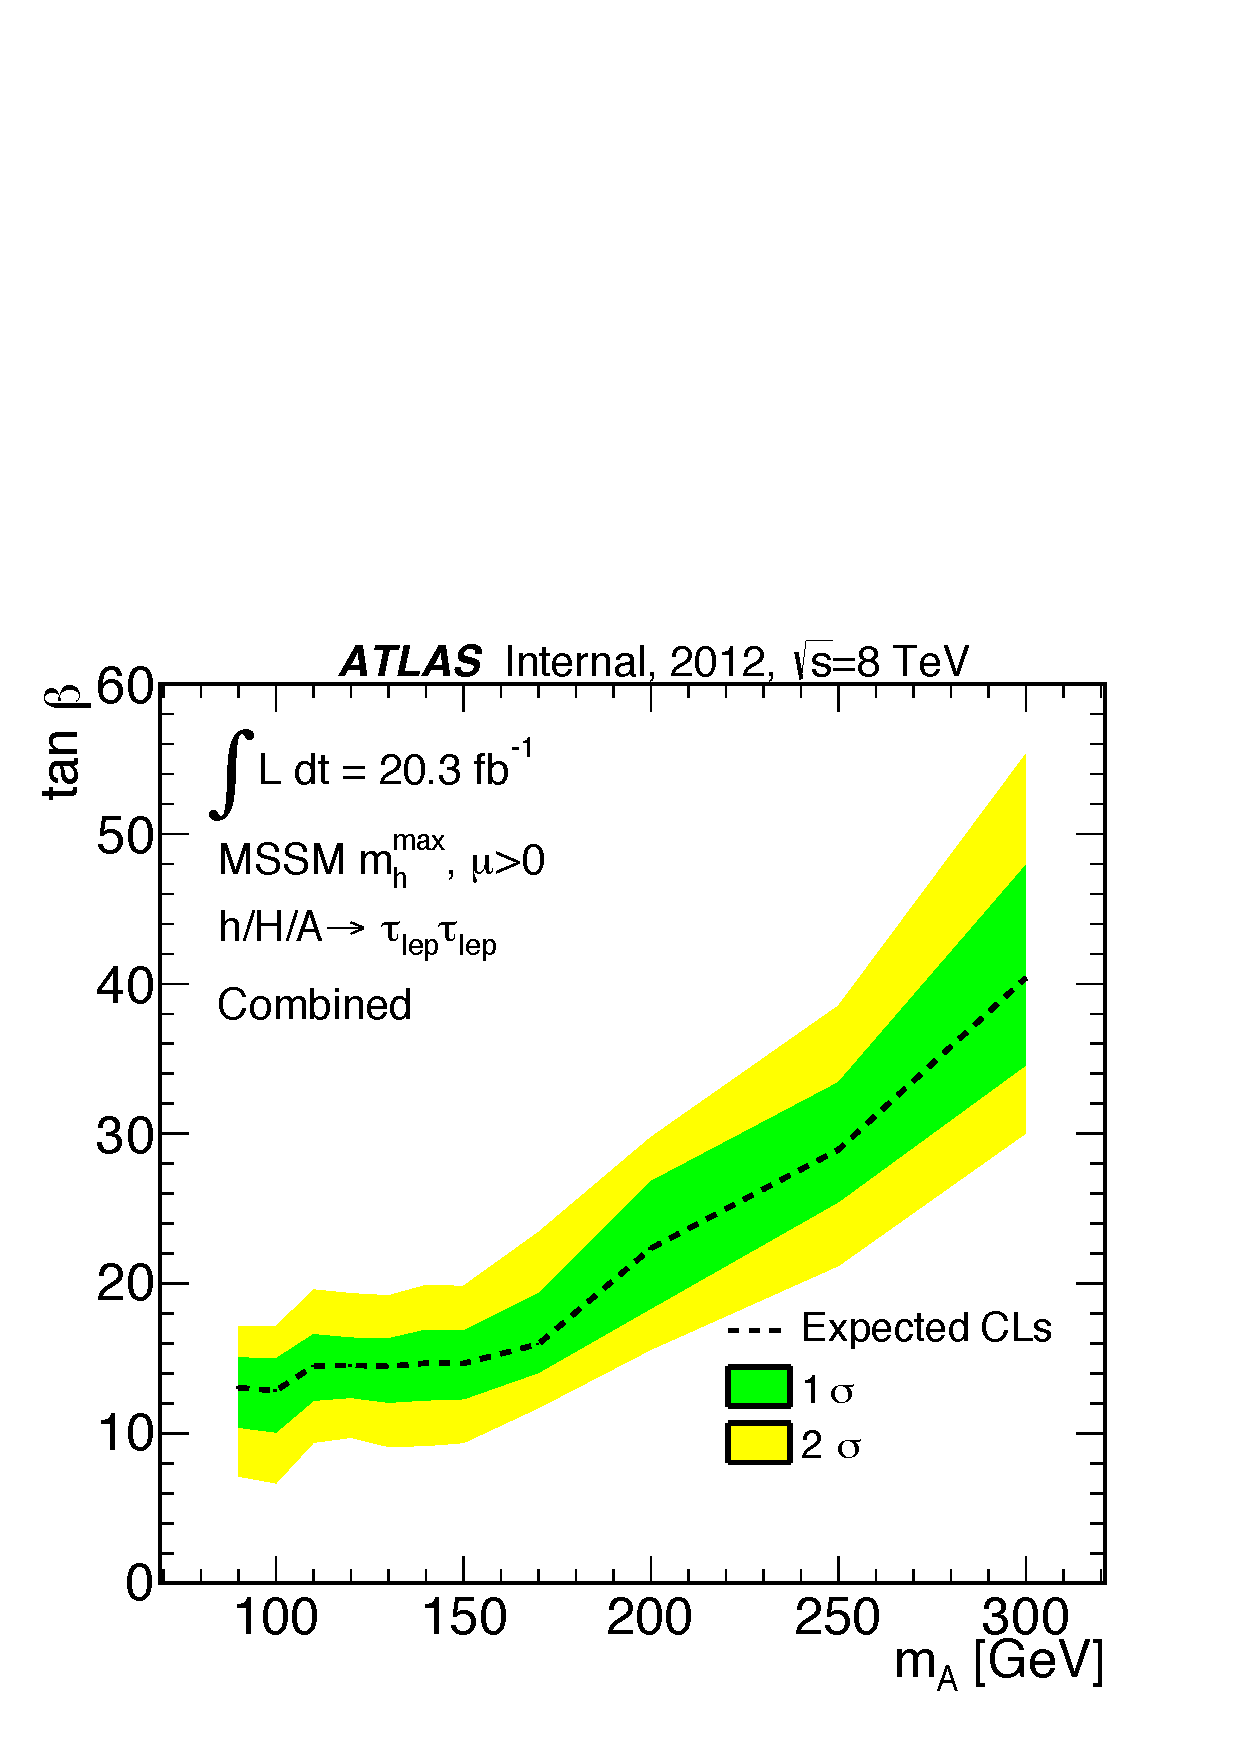
\includegraphics[width=0.65\textwidth]{figure/limits/Limits_mAtanBeta_Comb.pdf}
  \caption{Expected %and observed 
  exclusion limits for MSSM Higgs boson production 
in the MSSM $m_A$ vs $\tan\beta$ parameter space. Combination between b-tagged and b-vetoed category.}
\label{fig:limit_extract_combined}
\end{figure}


The outcome of the search is also interpreted in the generic case of a scalar boson produced in the
$pp \rightarrow gg \rightarrow \phi$ or $pp \rightarrow bb\phi$ mode and decaying to a di-tau pair.
The expected and observed $95\%$ confidence-level $CL_s$  limits on the cross section for the production of 
a generic Higgs boson $\phi$ are shown in Figure~\ref{fig:limit_xs}, 
the b-associated  and the gluon-gluon fusion production mechanisms are shown separately.
All signal systematic uncertainties are implemented in the likelihood
for this limit derivation, more information about the limits and their validation can be found in Appendix~\ref{appendix:limit}.

\begin{figure}[tp]
  \centering
% \includegraphics[width=0.45\textwidth]{}
% \includegraphics[width=0.45\textwidth]{}
  \caption{ Limits on the production of a scalar particle decaying to a di-tau pair
    and produced     in association with b quarks (left) or   via gluon-gluon fusion (right). Still not produced...}
\label{fig:limit_xs}
\end{figure}

